% \begin{figure}[htp]
% \begin{center}
% 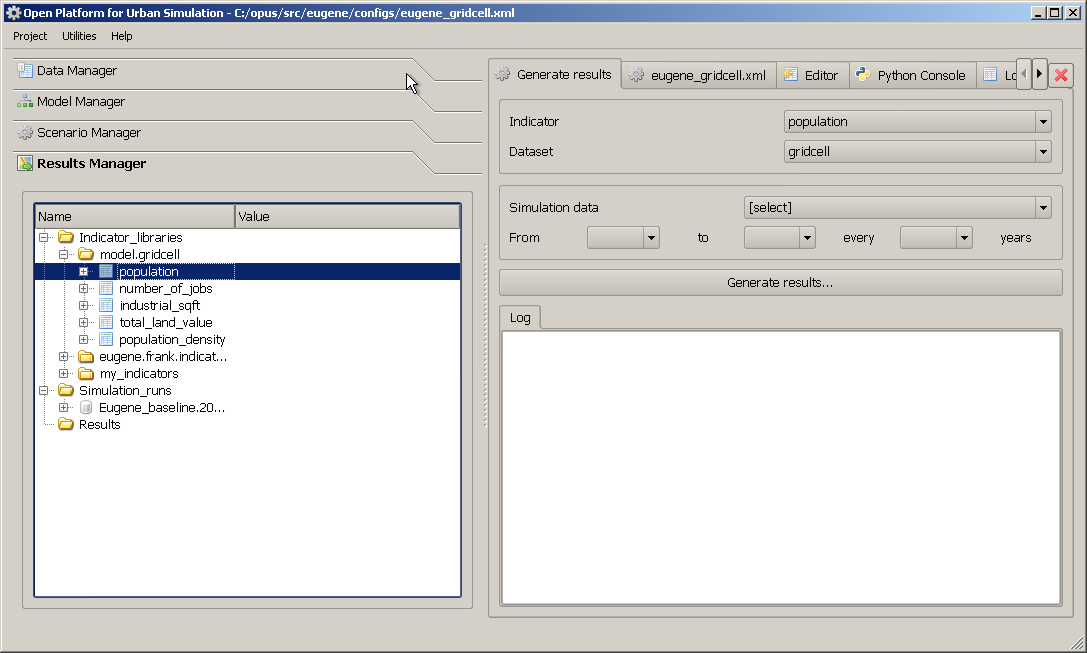
\includegraphics[scale=0.4]{graphics/opus-generate-indicator.png}
% \end{center}
% \caption{Generating an Indicator in the Results Manager}
% \label{fig:opus-generate-indicator}
% \end{figure}


\chapter{The Results Manager}

The Results Manager, corresponding to the Results tab of the GUI, has
two main responsibilities: to manage simulation runs for this project
and to allow the interrogation of these simulation results through
the use of \emph{indicators}. We explore both of these in this
chapter.

\section{Managing simulation runs}

[get run info]
[remove run and delete from harddrive]
[import run from disk]


\section{Interrogating results with Indicators}

Indicators are variables defined explicitly
for use as a meaningful measure. Like model variables, they can be
defined using the domain-specific programming language via the
``Variable Library'' item in the Tools menu. (XXX: forward pointer to
indicator chapter). An indicator can then be visualized as either a
map or as a table (the raw data) in a variety of formats. 

The GUI provides two ways to use indicators to understand what has
happened in your simulation:
\begin{enumerate}
  \item Interactive result exploration
  \item Batch indicator configuration and execution
\end{enumerate} 

\subsection{Interactive result exploration}

Often, it is desirable to explore your results in a lightweight
fashion in order to get a basic idea of what happened. You don't
necessarily want to go through the process of exporting results to a
GIS mapping tool in order to gain some intuition. 

The Opus GUI's \verb#Result Browser#, available from the \verb#tools#
menu, allows interactive exploration of simulation results. The Result
Browser presents a selectable list of available simulation runs, years
over which those simulations were run, and available indicators. You
can then configure an indicator visualization by selecting a simulation
run, a year, and an indicator. To compute and visualize the configured
indicator, simply press the \verb#generate results# button. The
indicator will then be computed for the year of the selected simulation
run. After it is computed, a tab should appear at the bottom of the
window with the name of the indicator and provide the ability to
visualize the results as a table or map (using the MatplotLib Python
module). See the inset tutorial XXX to try out the \verb#Result Browser#.

\fbox{
\begin{minipage}{.5\linewidth}
\begin{enumerate}
  \item Open the Results Browser from the Tools menu. Use the
  Results Browser to answer the following questions.
  \item Just from visual inspection, is there more than one
  cluster of gridcells with high land value in the Eugene region in 1980 in the baseyear data?
  \item Is this cluster(s) in the same general area as the
  greatest number of jobs in Eugene for the same year of the
  baseyear data?
\end{enumerate}
\end{minipage}
}

Two additional aspects of the Result Browser should be mentioned:
\begin{enumerate}
  \item If the checkbox \verb#Automatically view indicator# is
  clicked, everytime you change the indicator configuration (i.e.
  select a different simulation run, year, or indicator), the
  indicator will be automatically visualized (as if you pressed the
  \verb#Generate results# button). 
  \item The \verb#Export results# button will export the table data
  of the currently configured indicator to a database. This feature
  is not yet implemented. 
\end{enumerate}

\subsection{Batch indicator configuration and execution}

The \verb#Result Browser# is good for poking around in the
data. But often you'll want to generate the same
set of indicators for each of amny runs and you don't want to
redefine them every time. Instead, you'd like to configure and save a
group of them that can be executed on demand on an arbitrary
simulation run. In the Opus GUI, this functionality is supported with
\emph{indicator batches}. 

To create a new indicator batch, right-click on the
\verb#Indicator_batches# node in the \verb#Results tab# and select
\verb#Add new indicator batch...#. A new batch will be created
under the Indicator_batches node. You can rename the new batch if you
want by double-clicking its name and typing in a new one.

A batch is a collection of \verb#Indicator visualization#
definitions. Each indicator visualization is a configuration of
the indicator variable to be used, a visualization style (e.g. map or
table), and some format options. To add a new indicator visualization
to the batch, right-click on the respective batch and select
\verb#Add new indicator visualization...#. A dialog box will
appear where you can define the visualization. The visualization
options for an indicator visualzation are discussed in depth later in
subsection~\ref{sect:indicator-visualization-options}.

You can add as many indicator visualizations to a batch as you want.
In order to execute an indicator batch on a simulation run,
right-click on the indicator batch and hover over
 \verb#Run indicator batch on...#. A list of all the available 
 simulations runs will
appear as a submenu. You can then select the appropriate simulation
and the indicator visualizations in the batch will be executed over
all the years of that simulation run. If the resulting indicators are
tables or maps stored in a file, they can then be found on disk in
your \verb#OPUSHOME/data/PROJECTNAME/runs/RUNNAME/indicators#
directory, where \verb#PROJECTNAME# is the name of your project (e.g.
``eugene\_gridcell'') and \verb#RUNNAME# is the name of the
simulation run that you selected to run the batch on. The indicator
visualizations configured to write to a database will have produced
tables in the specified database with the name of the respective
indicator visualization. 


\subsubsection{Indicator visualization configuration options}
\label{sect:indicator-visualization-options}

Opus provides a rich variety of ways to visualize indicators and this
functionality is exposed in the \verb#Indicator visualization# dialog
box options (e.g. multi-year indicators, exporting to
databases). Unfortunately, this functionality can sometimes be hard
to present in an intuitive fashion. This section describes the range
of available options in the Batch indicator visualization dialog
box, which is separated into three components: ``indicator
selection'', ``output options'', and ``format options''. 

\heading{Indicator selection}

The bottom of the dialog box has two list boxes, ``available
indicators'' and ``indicators in current visualization''. The
indicators here are those variables from the \verb#Variable Library#
(XXX reference to variable library section) whose \emph{use} has been
set to be \emph{indicator} or \emph{both}. Note that the set of
indicators available is filtered by the currently selected dataset in
the ``output options'' (described later in this section).

By moving an indicator from the ``available indicators'' box to the
``indicators in current visualization'' box via the ``+'' button, you
include that indicator in this indicator visualization. Likewise, to
remove an indicator from the visualization, select the indicator in
the ``indicators in current visualization'' box and press the ``-''
button.


\heading{Output options}

\emph{Visualization Name}. The base name of any produced
visualizations. Because you might be producing this visualization for
different years and different simulation data, more information wil
be appended to this name to ensure uniqueness of the resulting file
or database table when the visualization is run on some data. 

\emph{Type}. There are two different types of indicator
visualizations that can be produced: maps and tables. Tables are just
raw data organized into rows and columns, while maps are
spatial projections of this data. The available format options
(described later) are fully dependent on the visualization type. 

\emph{Dataset name}. The dataset that this visualization corresponds
to. When the selected indicator(s) are run, they will be computed over
this dataset. Most commonly you are choosing a geographic granularity
(e.g. gridcell, zone) that you want to see the results at. Note that
when you change the dataset, the set of available indicators changes
because a given indicator is valid only for a single dataset.

\heading{Format options for maps}

The Matplotlib map is not intended to replace GIS-based mapping, which
allows far more control and the overlay of other features for visual
reference.  It is merely a quick tool to visualize data to get a sense
of the spatial patterns in it.  In order to support visualization in a
GIS environment such as ArcGIS or QGIS, the results may be exported to
a database or geodatabase environment, and the GIS software used to
create a more interactive and flexible display of the data.


\heading{Format options for tables}


[export results to database; geodatabase / autoview creation in
Postgres]



% 
% \subsection{Generating Indicators}
% 
% 
% 
% You will need to click the \verb#Simulation data# button and then
% select the simulation results you want to use.  Notice that the name of
% the scenario contains a date and time when the run was started.  Once
% you click on the \verb#Generate results# button, the indicator is
% computed.  A message is printed to the log, below the button, and a new
% entry will show up in the results node in the Results Manager tab on
% the left, as shown in Figure \ref{fig:opus-indicator-2}.
% 
% \begin{figure}[htp]
% \begin{center}
% 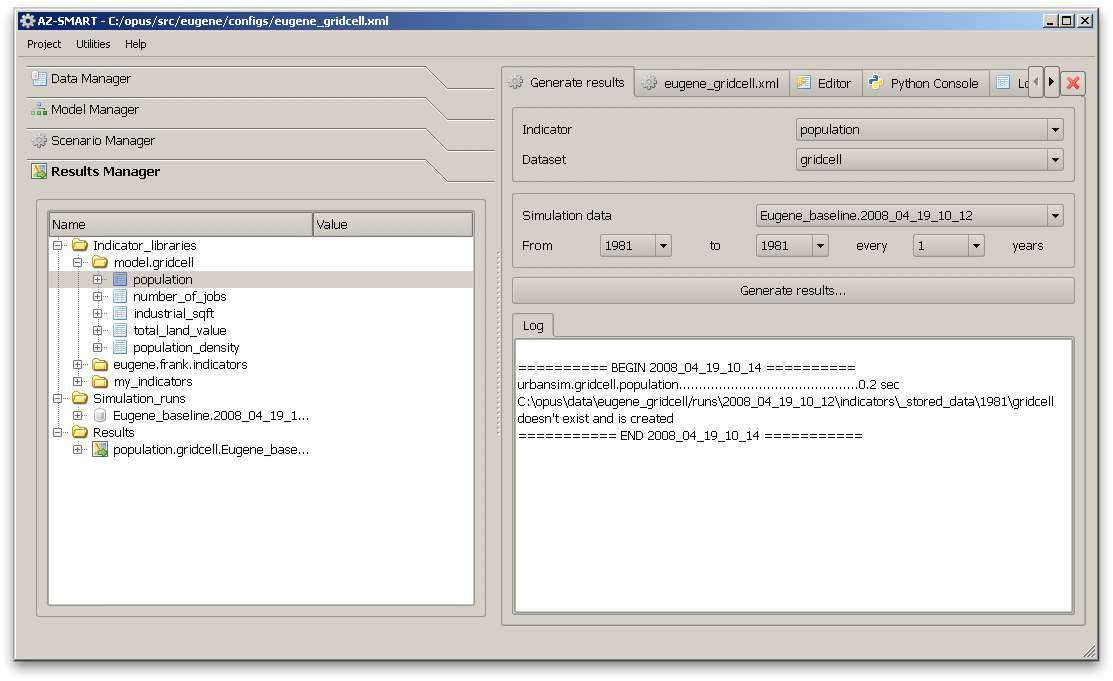
\includegraphics[scale=0.4]{graphics/opus-indicator-2.png}
% \end{center}
% \caption{Result of Generating an Indicator}
% \label{fig:opus-indicator-2}
% \end{figure}
% 
% Now that an indicator has been computed, its data is available to
% visualize or export to another application.  The Results Manager
% currently supports several ways to visualize an indicator, and these
% will depend on the nature of the indicator.  The menu for this is shown
% in Figure \ref{fig:opus-indicator-view-1}.  For example, the indicator
% that has just been computed is population by gridcell.  It is possible
% to visualize data on a grid using a simple image map, displayed on the
% right hand window using the Matplotlib Python library.   If you select
% the Map (Matplotlib) option on the menu, it will generate a map such as
% the one shown in Figure \ref{fig:opus-indicator-view-2}.
% 
% \begin{figure}[htp]
% \begin{center}
% 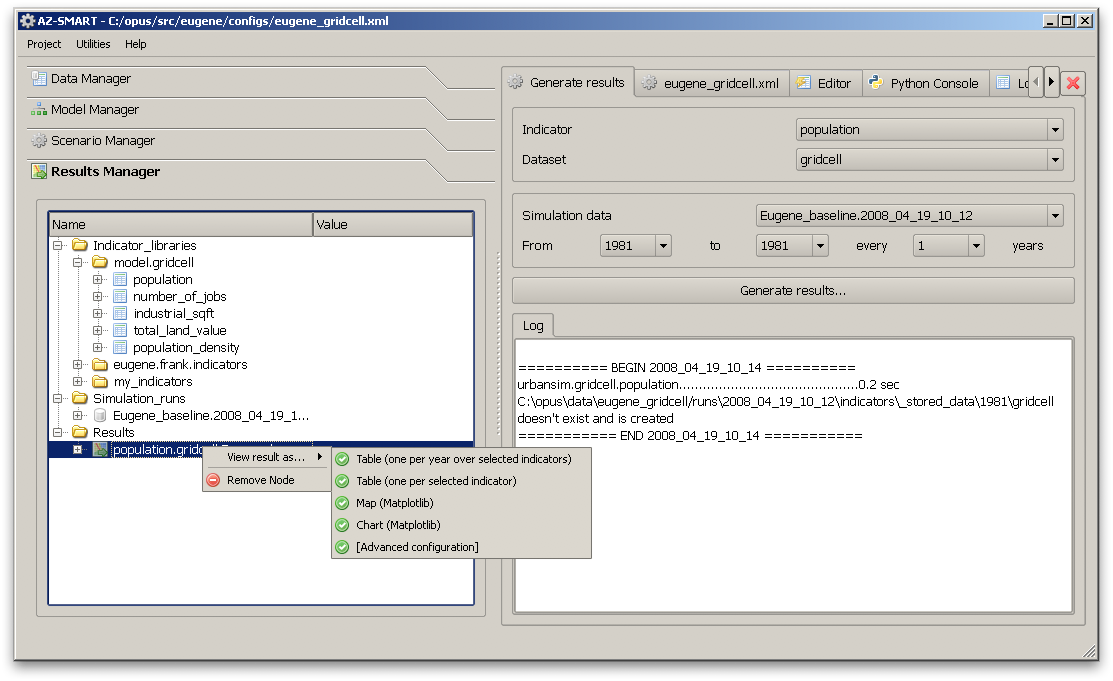
\includegraphics[scale=0.4]{graphics/opus-indicator-view-1.png}
% \end{center}
% \caption{View Results for an Indicator}
% \label{fig:opus-indicator-view-1}
% \end{figure}
% 
% \begin{figure}[htp]
% \begin{center}
% 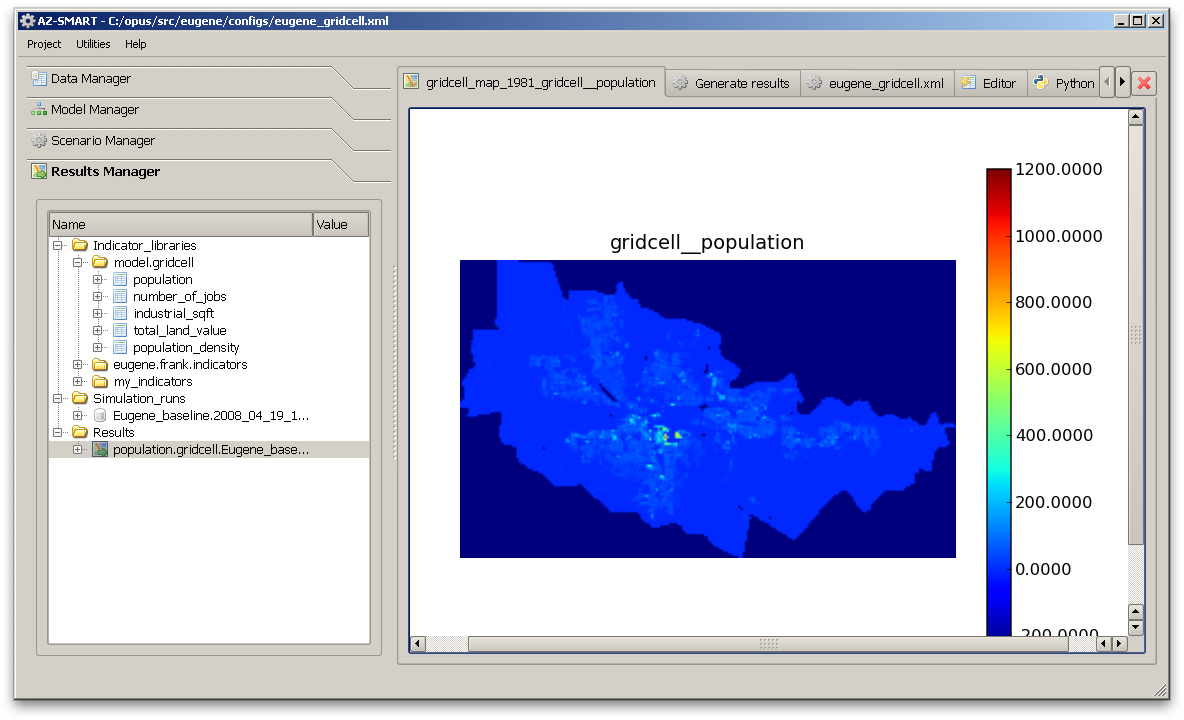
\includegraphics[scale=0.4]{graphics/opus-indicator-view-2.png}
% \end{center}
% \caption{Matplotlib Map for Population by Gridcell in Eugene-Springfield in 1981}
% \label{fig:opus-indicator-view-2}
% \end{figure}
% 
% The Matplotlib map is not intended to replace GIS-based mapping, which
% allows far more control and the overlay of other features for visual
% reference.  It is merely a quick tool to visualize data to get a sense
% of the spatial patterns in it.  In order to support visualization in a
% GIS environment such as ArcGIS or QGIS, the results may be exported to
% a database or geodatabase environment, and the GIS software used to
% create a more interactive and flexible display of the data.
% 
